% !TEX TS-program = pdflatex
% !TEX encoding = UTF-8 Unicode

%************************************************
\chapter{\textit{Appendice}}
\label{chp:Appendice}
%************************************************
\section*{\textit{Appendice 1}: Gesti legati ad un universo percussivo}

Prima di annotare l’analisi precedentemente fatta, ho cercato di tirar fuori una piccola analisi legata a gesti percussivi, evolvendo quello che avevo provato a fare due anni fa con lo Sp.I.R.E.. Ma purtroppo non ho ricevuto i risultati sperati. Il timbro, molto vicino ad una semplice ripresa di una molla a trazione, non rende possibile apprezzare tutte le capacità timbriche e strumentali di Unamolla. \\
Anzi, l’utilizzo di \textit{fff} o di avvicinamenti repentini della molla al legno\footnote{il parametro \textit{tensione} precedentemente sviscerato} può creare aberrazioni del segnale ed anche degli spiacevoli ticchettii, inadatti ad un universo compositivo ben definito. 
Di seguito degli spettrogrammi e spettro-frequenze, che fanno capire tali gesti.
\begin{itemize}
\item{\textbf{Analisi N. 7}: Colpo con mallet di legno \textit{mf}.}
\item{Analisi dello spettrogramma con ascisse in frequenza.}
\item{\textbf{Ripresa}: Somma segnali humb. + piezo}
\item{\textbf{Window}: 4096 frame}
\end{itemize}

\begin{figure}

\begin{center}

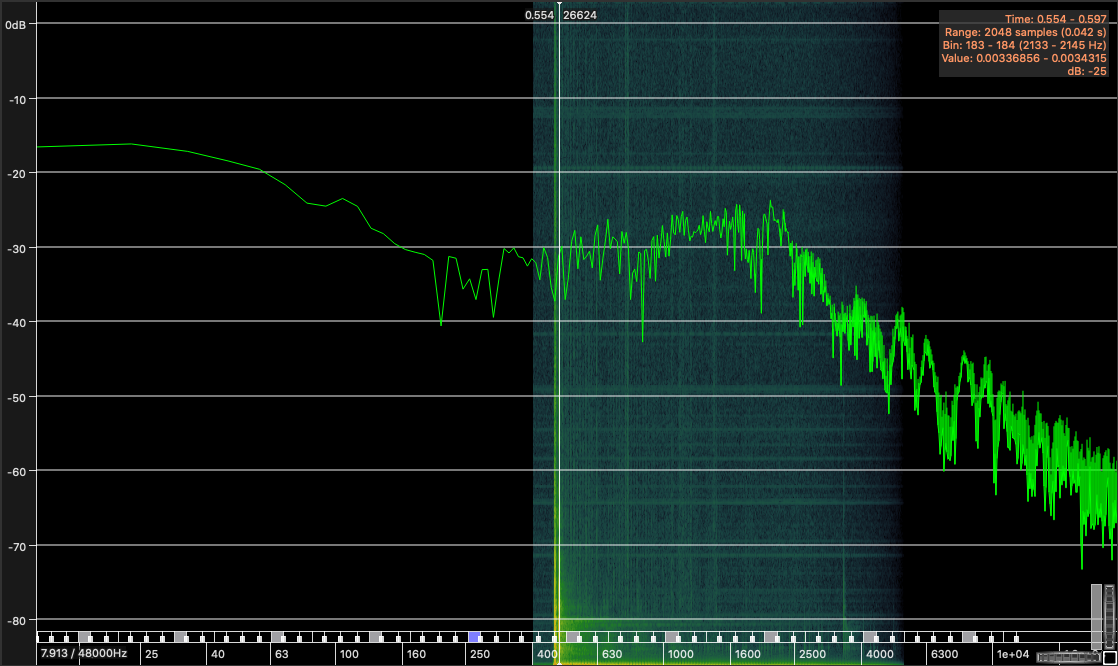
\includegraphics[width=1.\textwidth]{Unamolla_analisi_03.png}

\caption{Unamolla, Analisi n.7}

\label{fig:07_analisi_molla}

\end{center}

\end{figure}
\begin{itemize}
\item{\textbf{Analisi N. 8}: Colpo con mallet in ferro \textit{mf}.}
\item{Analisi dello spettrogramma con ascisse in frequenza.}
\item{textbf{Ripresa}: Somma segnali humb. + piezo.}
\item{textbf{Windowed}: 4096 frame.}
\end{itemize}

\begin{figure}

\begin{center}

\includegraphics[width=1.\textwidth]{Unamolla_analisi_04.png}

\caption{Unamolla, Analisi n.8}

\label{fig:08_analisi_molla}

\end{center}

\end{figure}
\begin{itemize}
\item{textbf{Analisi N. 9}: Grattato corto textit{mf}.}
\item{Analisi dello spettrogramma con ascisse in frequenza.}
\item{textbf{Ripresa}: Somma segnali humb. + piezo.}
\item{textbf{Window}: 4096 frame}
\end{itemize}

\begin{figure}

\begin{center}

\includegraphics[width=1.\textwidth]{Unamolla_analisi_05.png}

\caption{Unamolla, Analisi n.9}

\label{fig:09_analisi_molla}

\end{center}

\end{figure}
\begin{itemize}
\item{\textbf{Analisi N.10}: Grattato largo \textit{mf}.}
\item{Analisi dello spettrogramma con ascisse in frequenza.}
\item{\textbf{Ripresa}: Somma segnali humb. + piezo.}
\item{\textbf{Window}: 4096 frame.}
\end{itemize}

\begin{figure}

\begin{center}

\includegraphics[width=1.\textwidth]{Unamolla_analisi_06.png}

\caption{Unamolla, Analisi n.10}

\label{fig:10_analisi_molla}

\end{center}

\end{figure}

\begin{itemize}
\item{\textbf{Analisi N. 11}: Grattato tenuto \textit{mf}.}
\item{Analisi dello spettrogramma con ascisse in frequenza.}
\item{\textbf{Ripresa}: Somma segnali humb. + piezo.}
\item{\textbf{Windowed}: 4096 frame.}
\end{itemize}

\begin{figure}

\begin{center}

\includegraphics[width=1.\textwidth]{Unamolla_analisi_07.png}

\caption{Unamolla, Analisi n.11}

\label{fig:11_analisi_molla}

\end{center}

\end{figure}


\section*{Conclusioni}

Utilizzando mallet in ferro o l’archetto del violoncello, per quanto si risaltino un certo numero di armoniche, gli spettri rimangono con un MCD a 1. \\
Molti strumenti musicali, soprattutto nella categoria delle percussioni, hanno avuto un lungo percorso culturale prima di diventare dei veri e propri strumenti musicali. Tuttavia, non hanno avuto neppure poche modifiche e metamorfosi sia nello spettro che nell’aspetto, durante gli anni, che hanno portano a far sì che tali strumenti fossero catalogati come armonici. Grazie all’analisi, sia gestuale che spettrografica, si possono notare delle mancanze (ad esempio di una cassa di risonanza) che ha Unamolla. Di seguito vi , Grazie all’analisi si può notare che lo spettro si arricchisce di armonici se si utilizzano dei mallett in ferro o degli archetti per strumenti a corda e si fanno delle arcate corte. Così il suono è libero di propagarsi all’interno e all’esterno della molla. Inoltre, se si fa un’analisi completa dello spettro, notiamo che ci sono delle parziali, soprattutto nei casi di pizzicati e arcate corte. Se andiamo ad analizzare meglio la figura successiva, possiamo vedere come potrebbe essere eventualmente un prototipo diUnamolla 2.0 e di come sia possibile creare anche una cassa armonica variabile.
Al momento tutto ciò è solo un progetto quindi, tramite varie elaborazioni di elettronica come la creazione di filtri risonanti o di risonatori tramite micro-ritardi e feedback, possiamo arrivare ad avvicinare il suono al risultato voluto. 




